\documentclass[1p]{elsarticle_modified}
%\bibliographystyle{elsarticle-num}

%\usepackage[colorlinks]{hyperref}
%\usepackage{abbrmath_seonhwa} %\Abb, \Ascr, \Acal ,\Abf, \Afrak
\usepackage{amsfonts}
\usepackage{amssymb}
\usepackage{amsmath}
\usepackage{amsthm}
\usepackage{scalefnt}
\usepackage{amsbsy}
\usepackage{kotex}
\usepackage{caption}
\usepackage{subfig}
\usepackage{color}
\usepackage{graphicx}
\usepackage{xcolor} %% white, black, red, green, blue, cyan, magenta, yellow
\usepackage{float}
\usepackage{setspace}
\usepackage{hyperref}

\usepackage{tikz}
\usetikzlibrary{arrows}

\usepackage{multirow}
\usepackage{array} % fixed length table
\usepackage{hhline}

%%%%%%%%%%%%%%%%%%%%%
\makeatletter
\renewcommand*\env@matrix[1][\arraystretch]{%
	\edef\arraystretch{#1}%
	\hskip -\arraycolsep
	\let\@ifnextchar\new@ifnextchar
	\array{*\c@MaxMatrixCols c}}
\makeatother %https://tex.stackexchange.com/questions/14071/how-can-i-increase-the-line-spacing-in-a-matrix
%%%%%%%%%%%%%%%

\usepackage[normalem]{ulem}

\newcommand{\msout}[1]{\ifmmode\text{\sout{\ensuremath{#1}}}\else\sout{#1}\fi}
%SOURCE: \msout is \stkout macro in https://tex.stackexchange.com/questions/20609/strikeout-in-math-mode

\newcommand{\cancel}[1]{
	\ifmmode
	{\color{red}\msout{#1}}
	\else
	{\color{red}\sout{#1}}
	\fi
}

\newcommand{\add}[1]{
	{\color{blue}\uwave{#1}}
}

\newcommand{\replace}[2]{
	\ifmmode
	{\color{red}\msout{#1}}{\color{blue}\uwave{#2}}
	\else
	{\color{red}\sout{#1}}{\color{blue}\uwave{#2}}
	\fi
}

\newcommand{\Sol}{\mathcal{S}} %segment
\newcommand{\D}{D} %diagram
\newcommand{\A}{\mathcal{A}} %arc


%%%%%%%%%%%%%%%%%%%%%%%%%%%%%5 test

\def\sl{\operatorname{\textup{SL}}(2,\Cbb)}
\def\psl{\operatorname{\textup{PSL}}(2,\Cbb)}
\def\quan{\mkern 1mu \triangleright \mkern 1mu}

\theoremstyle{definition}
\newtheorem{thm}{Theorem}[section]
\newtheorem{prop}[thm]{Proposition}
\newtheorem{lem}[thm]{Lemma}
\newtheorem{ques}[thm]{Question}
\newtheorem{cor}[thm]{Corollary}
\newtheorem{defn}[thm]{Definition}
\newtheorem{exam}[thm]{Example}
\newtheorem{rmk}[thm]{Remark}
\newtheorem{alg}[thm]{Algorithm}

\newcommand{\I}{\sqrt{-1}}
\begin{document}

%\begin{frontmatter}
%
%\title{Boundary parabolic representations of knots up to 8 crossings}
%
%%% Group authors per affiliation:
%\author{Yunhi Cho} 
%\address{Department of Mathematics, University of Seoul, Seoul, Korea}
%\ead{yhcho@uos.ac.kr}
%
%
%\author{Seonhwa Kim} %\fnref{s_kim}}
%\address{Center for Geometry and Physics, Institute for Basic Science, Pohang, 37673, Korea}
%\ead{ryeona17@ibs.re.kr}
%
%\author{Hyuk Kim}
%\address{Department of Mathematical Sciences, Seoul National University, Seoul 08826, Korea}
%\ead{hyukkim@snu.ac.kr}
%
%\author{Seokbeom Yoon}
%\address{Department of Mathematical Sciences, Seoul National University, Seoul, 08826,  Korea}
%\ead{sbyoon15@snu.ac.kr}
%
%\begin{abstract}
%We find all boundary parabolic representation of knots up to 8 crossings.
%
%\end{abstract}
%\begin{keyword}
%    \MSC[2010] 57M25 
%\end{keyword}
%
%\end{frontmatter}

%\linenumbers
%\tableofcontents
%
\newcommand\colored[1]{\textcolor{white}{\rule[-0.35ex]{0.8em}{1.4ex}}\kern-0.8em\color{red} #1}%
%\newcommand\colored[1]{\textcolor{white}{ #1}\kern-2.17ex	\textcolor{white}{ #1}\kern-1.81ex	\textcolor{white}{ #1}\kern-2.15ex\color{red}#1	}

{\Large $\underline{12a_{1216}~(K12a_{1216})}$}

\setlength{\tabcolsep}{10pt}
\renewcommand{\arraystretch}{1.6}
\vspace{1cm}\begin{tabular}{m{100pt}>{\centering\arraybackslash}m{274pt}}
\multirow{5}{120pt}{
	\centering
	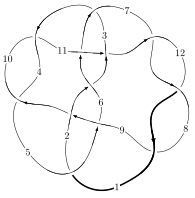
\includegraphics[width=112pt]{../../../GIT/diagram.site/Diagrams/png/2017_12a_1216.png}\\
\ \ \ A knot diagram\footnotemark}&
\allowdisplaybreaks
\textbf{Linearized knot diagam} \\
\cline{2-2}
 &
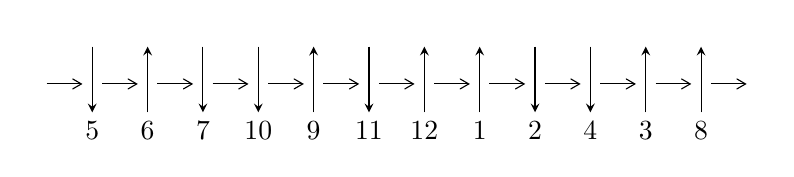
\begin{tikzpicture}[x=20pt, y=17pt]
	% nodes
	\node (C0) at (0, 0) {};
	\node (C1) at (1, 0) {};
	\node (C1U) at (1, +1) {};
	\node (C1D) at (1, -1) {5};

	\node (C2) at (2, 0) {};
	\node (C2U) at (2, +1) {};
	\node (C2D) at (2, -1) {6};

	\node (C3) at (3, 0) {};
	\node (C3U) at (3, +1) {};
	\node (C3D) at (3, -1) {7};

	\node (C4) at (4, 0) {};
	\node (C4U) at (4, +1) {};
	\node (C4D) at (4, -1) {10};

	\node (C5) at (5, 0) {};
	\node (C5U) at (5, +1) {};
	\node (C5D) at (5, -1) {9};

	\node (C6) at (6, 0) {};
	\node (C6U) at (6, +1) {};
	\node (C6D) at (6, -1) {11};

	\node (C7) at (7, 0) {};
	\node (C7U) at (7, +1) {};
	\node (C7D) at (7, -1) {12};

	\node (C8) at (8, 0) {};
	\node (C8U) at (8, +1) {};
	\node (C8D) at (8, -1) {1};

	\node (C9) at (9, 0) {};
	\node (C9U) at (9, +1) {};
	\node (C9D) at (9, -1) {2};

	\node (C10) at (10, 0) {};
	\node (C10U) at (10, +1) {};
	\node (C10D) at (10, -1) {4};

	\node (C11) at (11, 0) {};
	\node (C11U) at (11, +1) {};
	\node (C11D) at (11, -1) {3};

	\node (C12) at (12, 0) {};
	\node (C12U) at (12, +1) {};
	\node (C12D) at (12, -1) {8};
	\node (C13) at (13, 0) {};

	% arrows
	\draw[->,>={angle 60}]
	(C0) edge (C1) (C1) edge (C2) (C2) edge (C3) (C3) edge (C4) (C4) edge (C5) (C5) edge (C6) (C6) edge (C7) (C7) edge (C8) (C8) edge (C9) (C9) edge (C10) (C10) edge (C11) (C11) edge (C12) (C12) edge (C13) ;	\draw[->,>=stealth]
	(C1U) edge (C1D) (C2D) edge (C2U) (C3U) edge (C3D) (C4U) edge (C4D) (C5D) edge (C5U) (C6U) edge (C6D) (C7D) edge (C7U) (C8D) edge (C8U) (C9U) edge (C9D) (C10U) edge (C10D) (C11D) edge (C11U) (C12D) edge (C12U) ;
	\end{tikzpicture} \\
\hhline{~~} \\& 
\textbf{Solving Sequence} \\ \cline{2-2} 
 &
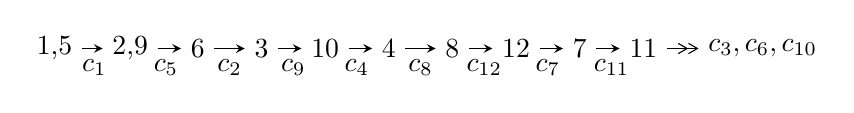
\begin{tikzpicture}[x=23pt, y=7pt]
	% node
	\node (A0) at (-1/8, 0) {1,5};
	\node (A1) at (17/16, 0) {2,9};
	\node (A2) at (17/8, 0) {6};
	\node (A3) at (25/8, 0) {3};
	\node (A4) at (33/8, 0) {10};
	\node (A5) at (41/8, 0) {4};
	\node (A6) at (49/8, 0) {8};
	\node (A7) at (57/8, 0) {12};
	\node (A8) at (65/8, 0) {7};
	\node (A9) at (73/8, 0) {11};
	\node (C1) at (1/2, -1) {$c_{1}$};
	\node (C2) at (13/8, -1) {$c_{5}$};
	\node (C3) at (21/8, -1) {$c_{2}$};
	\node (C4) at (29/8, -1) {$c_{9}$};
	\node (C5) at (37/8, -1) {$c_{4}$};
	\node (C6) at (45/8, -1) {$c_{8}$};
	\node (C7) at (53/8, -1) {$c_{12}$};
	\node (C8) at (61/8, -1) {$c_{7}$};
	\node (C9) at (69/8, -1) {$c_{11}$};
	\node (A10) at (11, 0) {$c_{3},c_{6},c_{10}$};

	% edge
	\draw[->,>=stealth]	
	(A0) edge (A1) (A1) edge (A2) (A2) edge (A3) (A3) edge (A4) (A4) edge (A5) (A5) edge (A6) (A6) edge (A7) (A7) edge (A8) (A8) edge (A9) ;
	\draw[->>,>={angle 60}]	
	(A9) edge (A10);
\end{tikzpicture} \\ 

\end{tabular} \\

\footnotetext{
The image of knot diagram is generated by the software ``\textbf{Draw programme}" developed by Andrew Bartholomew(\url{http://www.layer8.co.uk/maths/draw/index.htm\#Running-draw}), where we modified some parts for our purpose(\url{https://github.com/CATsTAILs/LinksPainter}).
}\phantom \\ \newline 
\centering \textbf{Ideals for irreducible components\footnotemark of $X_{\text{par}}$} 
 
\begin{align*}
I^u_{1}&=\langle 
3.07110\times10^{55} u^{35}+3.11578\times10^{55} u^{34}+\cdots+1.21007\times10^{57} b-2.38367\times10^{57},\\
\phantom{I^u_{1}}&\phantom{= \langle  }-3.06823\times10^{57} u^{35}-8.48330\times10^{57} u^{34}+\cdots+2.92837\times10^{58} a-3.15010\times10^{57},\\
\phantom{I^u_{1}}&\phantom{= \langle  }u^{36}+3 u^{35}+\cdots+31 u+11\rangle \\
I^u_{2}&=\langle 
1.96215\times10^{378} u^{83}-5.73830\times10^{378} u^{82}+\cdots+2.31304\times10^{381} b+1.14245\times10^{383},\\
\phantom{I^u_{2}}&\phantom{= \langle  }-2.55618\times10^{383} u^{83}+1.36720\times10^{384} u^{82}+\cdots+3.72608\times10^{385} a-4.36737\times10^{387},\\
\phantom{I^u_{2}}&\phantom{= \langle  }u^{84}-6 u^{83}+\cdots+75402 u+16109\rangle \\
I^u_{3}&=\langle 
-1.41646\times10^{18} u^{23}-1.09158\times10^{19} u^{22}+\cdots+9.42892\times10^{19} b-2.23684\times10^{20},\\
\phantom{I^u_{3}}&\phantom{= \langle  }-2.41868\times10^{19} u^{23}-2.30045\times10^{19} u^{22}+\cdots+3.45727\times10^{20} a+9.65371\times10^{20},\\
\phantom{I^u_{3}}&\phantom{= \langle  }u^{24}+u^{23}+\cdots-44 u+11\rangle \\
I^u_{4}&=\langle 
- u^2+b+u-1,\;u^3- u^2+a+2 u,\;u^5- u^4+3 u^3+u+1\rangle \\
\\
\end{align*}
\raggedright * 4 irreducible components of $\dim_{\mathbb{C}}=0$, with total 149 representations.\\
\footnotetext{All coefficients of polynomials are rational numbers. But the coefficients are sometimes approximated in decimal forms when there is not enough margin.}
\newpage
\renewcommand{\arraystretch}{1}
\centering \section*{I. $I^u_{1}= \langle 3.07\times10^{55} u^{35}+3.12\times10^{55} u^{34}+\cdots+1.21\times10^{57} b-2.38\times10^{57},\;-3.07\times10^{57} u^{35}-8.48\times10^{57} u^{34}+\cdots+2.93\times10^{58} a-3.15\times10^{57},\;u^{36}+3 u^{35}+\cdots+31 u+11 \rangle$}
\flushleft \textbf{(i) Arc colorings}\\
\begin{tabular}{m{7pt} m{180pt} m{7pt} m{180pt} }
\flushright $a_{1}=$&$\begin{pmatrix}1\\0\end{pmatrix}$ \\
\flushright $a_{5}=$&$\begin{pmatrix}0\\u\end{pmatrix}$ \\
\flushright $a_{2}=$&$\begin{pmatrix}1\\u^2\end{pmatrix}$ \\
\flushright $a_{9}=$&$\begin{pmatrix}0.104776 u^{35}+0.289694 u^{34}+\cdots+8.06655 u+0.107572\\-0.0253796 u^{35}-0.0257488 u^{34}+\cdots+2.33690 u+1.96987\end{pmatrix}$ \\
\flushright $a_{6}=$&$\begin{pmatrix}-0.0430439 u^{35}-0.0980154 u^{34}+\cdots-1.26891 u+1.90110\\-0.0282150 u^{35}-0.0943192 u^{34}+\cdots-1.90756 u-0.940844\end{pmatrix}$ \\
\flushright $a_{3}=$&$\begin{pmatrix}0.0194838 u^{35}+0.0845787 u^{34}+\cdots+2.21756 u+2.39922\\-0.00642062 u^{35}-0.0145250 u^{34}+\cdots-0.611763 u-0.128826\end{pmatrix}$ \\
\flushright $a_{10}=$&$\begin{pmatrix}0.119201 u^{35}+0.286732 u^{34}+\cdots+5.34079 u-1.59131\\-0.0176093 u^{35}+0.0122805 u^{34}+\cdots+3.61154 u+2.47846\end{pmatrix}$ \\
\flushright $a_{4}=$&$\begin{pmatrix}-0.0321006 u^{35}-0.0871705 u^{34}+\cdots+1.07521 u+2.34185\\0.0515844 u^{35}+0.171749 u^{34}+\cdots+1.14236 u+0.0573708\end{pmatrix}$ \\
\flushright $a_{8}=$&$\begin{pmatrix}0.130156 u^{35}+0.315443 u^{34}+\cdots+5.72965 u-1.86229\\-0.0253796 u^{35}-0.0257488 u^{34}+\cdots+2.33690 u+1.96987\end{pmatrix}$ \\
\flushright $a_{12}=$&$\begin{pmatrix}0.0218056 u^{35}+0.0861969 u^{34}+\cdots+5.45506 u+0.366809\\0.0637256 u^{35}+0.142182 u^{34}+\cdots+0.735110 u+0.377098\end{pmatrix}$ \\
\flushright $a_{7}=$&$\begin{pmatrix}-0.00521553 u^{35}+0.0359378 u^{34}+\cdots+6.08640 u+0.980678\\0.0169269 u^{35}-0.00722416 u^{34}+\cdots-4.32230 u-1.22939\end{pmatrix}$ \\
\flushright $a_{11}=$&$\begin{pmatrix}-0.0405255 u^{35}-0.0987638 u^{34}+\cdots-0.0270432 u-1.57349\\0.0588225 u^{35}+0.139014 u^{34}+\cdots+1.58649 u+0.520172\end{pmatrix}$\\&\end{tabular}
\flushleft \textbf{(ii) Obstruction class $= -1$}\\~\\
\flushleft \textbf{(iii) Cusp Shapes $= 0.343599 u^{35}+0.938842 u^{34}+\cdots+7.99255 u+3.25096$}\\~\\
\newpage\renewcommand{\arraystretch}{1}
\flushleft \textbf{(iv) u-Polynomials at the component}\newline \\
\begin{tabular}{m{50pt}|m{274pt}}
Crossings & \hspace{64pt}u-Polynomials at each crossing \\
\hline $$\begin{aligned}c_{1},c_{3}\end{aligned}$$&$\begin{aligned}
&u^{36}-3 u^{35}+\cdots-31 u+11
\end{aligned}$\\
\hline $$\begin{aligned}c_{2}\end{aligned}$$&$\begin{aligned}
&u^{36}-7 u^{35}+\cdots-12071 u+1268
\end{aligned}$\\
\hline $$\begin{aligned}c_{4},c_{10}\end{aligned}$$&$\begin{aligned}
&11(11 u^{36}-27 u^{35}+\cdots-224 u+64)
\end{aligned}$\\
\hline $$\begin{aligned}c_{5},c_{11}\end{aligned}$$&$\begin{aligned}
&11(11 u^{36}-5 u^{35}+\cdots+11 u+1)
\end{aligned}$\\
\hline $$\begin{aligned}c_{6},c_{9}\end{aligned}$$&$\begin{aligned}
&u^{36}+u^{35}+\cdots+17 u+11
\end{aligned}$\\
\hline $$\begin{aligned}c_{7},c_{8},c_{12}\end{aligned}$$&$\begin{aligned}
&u^{36}+4 u^{35}+\cdots-71 u+28
\end{aligned}$\\
\hline
\end{tabular}\\~\\
\newpage\renewcommand{\arraystretch}{1}
\flushleft \textbf{(v) Riley Polynomials at the component}\newline \\
\begin{tabular}{m{50pt}|m{274pt}}
Crossings & \hspace{64pt}Riley Polynomials at each crossing \\
\hline $$\begin{aligned}c_{1},c_{3}\end{aligned}$$&$\begin{aligned}
&y^{36}+17 y^{35}+\cdots+1525 y+121
\end{aligned}$\\
\hline $$\begin{aligned}c_{2}\end{aligned}$$&$\begin{aligned}
&y^{36}-5 y^{35}+\cdots-32055665 y+1607824
\end{aligned}$\\
\hline $$\begin{aligned}c_{4},c_{10}\end{aligned}$$&$\begin{aligned}
&121(121 y^{36}+4177 y^{35}+\cdots-52224 y+4096)
\end{aligned}$\\
\hline $$\begin{aligned}c_{5},c_{11}\end{aligned}$$&$\begin{aligned}
&121(121 y^{36}-179 y^{35}+\cdots-15 y+1)
\end{aligned}$\\
\hline $$\begin{aligned}c_{6},c_{9}\end{aligned}$$&$\begin{aligned}
&y^{36}-9 y^{35}+\cdots-993 y+121
\end{aligned}$\\
\hline $$\begin{aligned}c_{7},c_{8},c_{12}\end{aligned}$$&$\begin{aligned}
&y^{36}-42 y^{35}+\cdots-10025 y+784
\end{aligned}$\\
\hline
\end{tabular}\\~\\
\newpage\flushleft \textbf{(vi) Complex Volumes and Cusp Shapes}
$$\begin{array}{c|c|c}  
\text{Solutions to }I^u_{1}& \I (\text{vol} + \sqrt{-1}CS) & \text{Cusp shape}\\
 \hline 
\begin{aligned}
u &= \phantom{-}0.626439 + 0.821744 I \\
a &= -0.014200 + 0.915314 I \\
b &= \phantom{-}0.285946 + 1.359990 I\end{aligned}
 & \phantom{-}5.67717 - 7.19089 I & \phantom{-}6.77872 + 10.51894 I \\ \hline\begin{aligned}
u &= \phantom{-}0.626439 - 0.821744 I \\
a &= -0.014200 - 0.915314 I \\
b &= \phantom{-}0.285946 - 1.359990 I\end{aligned}
 & \phantom{-}5.67717 + 7.19089 I & \phantom{-}6.77872 - 10.51894 I \\ \hline\begin{aligned}
u &= -0.735513 + 0.847069 I \\
a &= -0.061617 - 1.306230 I \\
b &= -0.731247 - 0.579536 I\end{aligned}
 & \phantom{-}1.25199 + 9.16761 I & \phantom{-}2.00321 - 10.89319 I \\ \hline\begin{aligned}
u &= -0.735513 - 0.847069 I \\
a &= -0.061617 + 1.306230 I \\
b &= -0.731247 + 0.579536 I\end{aligned}
 & \phantom{-}1.25199 - 9.16761 I & \phantom{-}2.00321 + 10.89319 I \\ \hline\begin{aligned}
u &= \phantom{-}0.772732 + 0.874210 I \\
a &= \phantom{-}0.194851 + 0.728325 I \\
b &= -0.486450 + 0.481309 I\end{aligned}
 & -1.16285 - 3.35532 I & -5.76129 + 8.10680 I \\ \hline\begin{aligned}
u &= \phantom{-}0.772732 - 0.874210 I \\
a &= \phantom{-}0.194851 - 0.728325 I \\
b &= -0.486450 - 0.481309 I\end{aligned}
 & -1.16285 + 3.35532 I & -5.76129 - 8.10680 I \\ \hline\begin{aligned}
u &= -0.805692 + 0.116635 I \\
a &= \phantom{-}0.617278 - 1.109470 I \\
b &= \phantom{-}0.337006 - 0.262138 I\end{aligned}
 & \phantom{-}2.93111 - 1.00501 I & -2.25229 + 5.18116 I \\ \hline\begin{aligned}
u &= -0.805692 - 0.116635 I \\
a &= \phantom{-}0.617278 + 1.109470 I \\
b &= \phantom{-}0.337006 + 0.262138 I\end{aligned}
 & \phantom{-}2.93111 + 1.00501 I & -2.25229 - 5.18116 I \\ \hline\begin{aligned}
u &= -0.165485 + 0.766453 I \\
a &= \phantom{-}1.42439 - 0.22806 I \\
b &= -1.69610 + 0.07451 I\end{aligned}
 & \phantom{-}11.30080 + 0.97216 I & \phantom{-}1.38322 - 7.38671 I \\ \hline\begin{aligned}
u &= -0.165485 - 0.766453 I \\
a &= \phantom{-}1.42439 + 0.22806 I \\
b &= -1.69610 - 0.07451 I\end{aligned}
 & \phantom{-}11.30080 - 0.97216 I & \phantom{-}1.38322 + 7.38671 I\\
 \hline 
 \end{array}$$\newpage$$\begin{array}{c|c|c}  
\text{Solutions to }I^u_{1}& \I (\text{vol} + \sqrt{-1}CS) & \text{Cusp shape}\\
 \hline 
\begin{aligned}
u &= \phantom{-}0.696880 + 0.295020 I \\
a &= \phantom{-}0.096744 - 0.480185 I \\
b &= -0.400914 - 0.336417 I\end{aligned}
 & -1.319370 - 0.296330 I & -6.81999 - 0.16370 I \\ \hline\begin{aligned}
u &= \phantom{-}0.696880 - 0.295020 I \\
a &= \phantom{-}0.096744 + 0.480185 I \\
b &= -0.400914 + 0.336417 I\end{aligned}
 & -1.319370 + 0.296330 I & -6.81999 + 0.16370 I \\ \hline\begin{aligned}
u &= -0.737714 + 1.001740 I \\
a &= -0.073548 - 0.249450 I \\
b &= \phantom{-}0.589463 - 0.458452 I\end{aligned}
 & \phantom{-}2.89931 + 3.69822 I & \phantom{-}0.38877 - 1.68665 I \\ \hline\begin{aligned}
u &= -0.737714 - 1.001740 I \\
a &= -0.073548 + 0.249450 I \\
b &= \phantom{-}0.589463 + 0.458452 I\end{aligned}
 & \phantom{-}2.89931 - 3.69822 I & \phantom{-}0.38877 + 1.68665 I \\ \hline\begin{aligned}
u &= -0.405498 + 0.604340 I \\
a &= -0.253574 + 1.341290 I \\
b &= -0.285857 + 0.818526 I\end{aligned}
 & -0.18794 + 4.61110 I & -1.49697 - 10.53385 I \\ \hline\begin{aligned}
u &= -0.405498 - 0.604340 I \\
a &= -0.253574 - 1.341290 I \\
b &= -0.285857 - 0.818526 I\end{aligned}
 & -0.18794 - 4.61110 I & -1.49697 + 10.53385 I \\ \hline\begin{aligned}
u &= -0.018649 + 0.720074 I \\
a &= \phantom{-}0.212930 - 0.920994 I \\
b &= -2.00932 - 0.41237 I\end{aligned}
 & \phantom{-}12.86020 + 1.02559 I & \phantom{-}15.7606 - 6.4698 I \\ \hline\begin{aligned}
u &= -0.018649 - 0.720074 I \\
a &= \phantom{-}0.212930 + 0.920994 I \\
b &= -2.00932 + 0.41237 I\end{aligned}
 & \phantom{-}12.86020 - 1.02559 I & \phantom{-}15.7606 + 6.4698 I \\ \hline\begin{aligned}
u &= \phantom{-}0.570273 + 0.403483 I \\
a &= \phantom{-}0.797604 - 0.529762 I \\
b &= \phantom{-}1.71444 - 0.17611 I\end{aligned}
 & \phantom{-}6.75055 - 0.27364 I & \phantom{-}3.68665 + 13.40425 I \\ \hline\begin{aligned}
u &= \phantom{-}0.570273 - 0.403483 I \\
a &= \phantom{-}0.797604 + 0.529762 I \\
b &= \phantom{-}1.71444 + 0.17611 I\end{aligned}
 & \phantom{-}6.75055 + 0.27364 I & \phantom{-}3.68665 - 13.40425 I\\
 \hline 
 \end{array}$$\newpage$$\begin{array}{c|c|c}  
\text{Solutions to }I^u_{1}& \I (\text{vol} + \sqrt{-1}CS) & \text{Cusp shape}\\
 \hline 
\begin{aligned}
u &= -0.896164 + 1.034610 I \\
a &= \phantom{-}0.190031 + 1.352920 I \\
b &= \phantom{-}1.62048 + 0.16576 I\end{aligned}
 & \phantom{-}9.2208 + 11.9404 I & \phantom{-}5.14110 - 9.30022 I \\ \hline\begin{aligned}
u &= -0.896164 - 1.034610 I \\
a &= \phantom{-}0.190031 - 1.352920 I \\
b &= \phantom{-}1.62048 - 0.16576 I\end{aligned}
 & \phantom{-}9.2208 - 11.9404 I & \phantom{-}5.14110 + 9.30022 I \\ \hline\begin{aligned}
u &= -1.379280 + 0.100054 I \\
a &= -0.551599 + 0.192022 I \\
b &= -1.48860 - 0.03556 I\end{aligned}
 & \phantom{-}8.76113 - 1.33737 I & \phantom{-}5.81278 + 5.28943 I \\ \hline\begin{aligned}
u &= -1.379280 - 0.100054 I \\
a &= -0.551599 - 0.192022 I \\
b &= -1.48860 + 0.03556 I\end{aligned}
 & \phantom{-}8.76113 + 1.33737 I & \phantom{-}5.81278 - 5.28943 I \\ \hline\begin{aligned}
u &= \phantom{-}0.85971 + 1.17187 I \\
a &= -0.049347 - 0.951517 I \\
b &= \phantom{-}0.903388 - 0.869869 I\end{aligned}
 & \phantom{-}7.7128 - 14.1526 I & \phantom{-}5.37015 + 9.64601 I \\ \hline\begin{aligned}
u &= \phantom{-}0.85971 - 1.17187 I \\
a &= -0.049347 + 0.951517 I \\
b &= \phantom{-}0.903388 + 0.869869 I\end{aligned}
 & \phantom{-}7.7128 + 14.1526 I & \phantom{-}5.37015 - 9.64601 I \\ \hline\begin{aligned}
u &= -0.156302 + 0.359262 I \\
a &= -0.90151 + 1.91392 I \\
b &= \phantom{-}0.858883 + 0.215221 I\end{aligned}
 & \phantom{-}1.63286 + 0.71455 I & \phantom{-}2.07561 - 1.46762 I \\ \hline\begin{aligned}
u &= -0.156302 - 0.359262 I \\
a &= -0.90151 - 1.91392 I \\
b &= \phantom{-}0.858883 - 0.215221 I\end{aligned}
 & \phantom{-}1.63286 - 0.71455 I & \phantom{-}2.07561 + 1.46762 I \\ \hline\begin{aligned}
u &= \phantom{-}0.77773 + 1.43937 I \\
a &= -0.327351 - 0.665051 I \\
b &= \phantom{-}1.51996 - 0.13931 I\end{aligned}
 & \phantom{-}5.50525 - 5.57144 I & \phantom{-0.000000 } 0 \\ \hline\begin{aligned}
u &= \phantom{-}0.77773 - 1.43937 I \\
a &= -0.327351 + 0.665051 I \\
b &= \phantom{-}1.51996 + 0.13931 I\end{aligned}
 & \phantom{-}5.50525 + 5.57144 I & \phantom{-0.000000 } 0\\
 \hline 
 \end{array}$$\newpage$$\begin{array}{c|c|c}  
\text{Solutions to }I^u_{1}& \I (\text{vol} + \sqrt{-1}CS) & \text{Cusp shape}\\
 \hline 
\begin{aligned}
u &= \phantom{-}0.91981 + 1.44541 I \\
a &= \phantom{-}0.083609 + 0.983332 I \\
b &= -1.68386 + 0.26413 I\end{aligned}
 & \phantom{-}16.3072 - 18.5095 I & \phantom{-0.000000 } 0 \\ \hline\begin{aligned}
u &= \phantom{-}0.91981 - 1.44541 I \\
a &= \phantom{-}0.083609 - 0.983332 I \\
b &= -1.68386 - 0.26413 I\end{aligned}
 & \phantom{-}16.3072 + 18.5095 I & \phantom{-0.000000 } 0 \\ \hline\begin{aligned}
u &= -0.71477 + 1.57778 I \\
a &= -0.255474 + 0.443114 I \\
b &= \phantom{-}0.529759 + 0.323204 I\end{aligned}
 & \phantom{-}2.68916 + 6.34722 I & \phantom{-0.000000 } 0 \\ \hline\begin{aligned}
u &= -0.71477 - 1.57778 I \\
a &= -0.255474 - 0.443114 I \\
b &= \phantom{-}0.529759 - 0.323204 I\end{aligned}
 & \phantom{-}2.68916 - 6.34722 I & \phantom{-0.000000 } 0 \\ \hline\begin{aligned}
u &= -0.70851 + 2.00785 I \\
a &= \phantom{-}0.374916 - 0.443328 I \\
b &= -1.57698 - 0.08807 I\end{aligned}
 & \phantom{-}9.97824 + 7.80433 I & \phantom{-0.000000 } 0 \\ \hline\begin{aligned}
u &= -0.70851 - 2.00785 I \\
a &= \phantom{-}0.374916 + 0.443328 I \\
b &= -1.57698 + 0.08807 I\end{aligned}
 & \phantom{-}9.97824 - 7.80433 I & \phantom{-0.000000 } 0\\
 \hline 
 \end{array}$$\newpage\newpage\renewcommand{\arraystretch}{1}
\centering \section*{II. $I^u_{2}= \langle 1.96\times10^{378} u^{83}-5.74\times10^{378} u^{82}+\cdots+2.31\times10^{381} b+1.14\times10^{383},\;-2.56\times10^{383} u^{83}+1.37\times10^{384} u^{82}+\cdots+3.73\times10^{385} a-4.37\times10^{387},\;u^{84}-6 u^{83}+\cdots+75402 u+16109 \rangle$}
\flushleft \textbf{(i) Arc colorings}\\
\begin{tabular}{m{7pt} m{180pt} m{7pt} m{180pt} }
\flushright $a_{1}=$&$\begin{pmatrix}1\\0\end{pmatrix}$ \\
\flushright $a_{5}=$&$\begin{pmatrix}0\\u\end{pmatrix}$ \\
\flushright $a_{2}=$&$\begin{pmatrix}1\\u^2\end{pmatrix}$ \\
\flushright $a_{9}=$&$\begin{pmatrix}0.00686023 u^{83}-0.0366927 u^{82}+\cdots+770.784 u+117.211\\-0.000848300 u^{83}+0.00248085 u^{82}+\cdots-242.928 u-49.3918\end{pmatrix}$ \\
\flushright $a_{6}=$&$\begin{pmatrix}-0.0168256 u^{83}+0.122202 u^{82}+\cdots+1670.97 u+450.926\\0.00649536 u^{83}-0.0484208 u^{82}+\cdots-918.996 u-236.276\end{pmatrix}$ \\
\flushright $a_{3}=$&$\begin{pmatrix}0.0354912 u^{83}-0.232975 u^{82}+\cdots-748.044 u-335.703\\-0.0188856 u^{83}+0.133648 u^{82}+\cdots+1425.41 u+406.752\end{pmatrix}$ \\
\flushright $a_{10}=$&$\begin{pmatrix}0.00459288 u^{83}-0.0233944 u^{82}+\cdots+566.251 u+94.6163\\-0.000548050 u^{83}+0.000304096 u^{82}+\cdots-183.346 u-44.4657\end{pmatrix}$ \\
\flushright $a_{4}=$&$\begin{pmatrix}-0.0108581 u^{83}+0.0775995 u^{82}+\cdots+1106.74 u+294.456\\0.00419775 u^{83}-0.0306150 u^{82}+\cdots-609.826 u-150.118\end{pmatrix}$ \\
\flushright $a_{8}=$&$\begin{pmatrix}0.00770853 u^{83}-0.0391735 u^{82}+\cdots+1013.71 u+166.603\\-0.000848300 u^{83}+0.00248085 u^{82}+\cdots-242.928 u-49.3918\end{pmatrix}$ \\
\flushright $a_{12}=$&$\begin{pmatrix}0.0217802 u^{83}-0.121456 u^{82}+\cdots+1657.93 u+239.097\\-0.00711285 u^{83}+0.0399474 u^{82}+\cdots-415.961 u-52.1460\end{pmatrix}$ \\
\flushright $a_{7}=$&$\begin{pmatrix}-0.0111339 u^{83}+0.0504405 u^{82}+\cdots-2063.90 u-380.414\\0.00551466 u^{83}-0.0250079 u^{82}+\cdots+1064.17 u+192.856\end{pmatrix}$ \\
\flushright $a_{11}=$&$\begin{pmatrix}-0.0165383 u^{83}+0.0810880 u^{82}+\cdots-2538.50 u-468.124\\0.0147464 u^{83}-0.0845715 u^{82}+\cdots+1055.87 u+156.995\end{pmatrix}$\\&\end{tabular}
\flushleft \textbf{(ii) Obstruction class $= -1$}\\~\\
\flushleft \textbf{(iii) Cusp Shapes $= 0.0487492 u^{83}-0.270054 u^{82}+\cdots+2871.27 u+426.180$}\\~\\
\newpage\renewcommand{\arraystretch}{1}
\flushleft \textbf{(iv) u-Polynomials at the component}\newline \\
\begin{tabular}{m{50pt}|m{274pt}}
Crossings & \hspace{64pt}u-Polynomials at each crossing \\
\hline $$\begin{aligned}c_{1},c_{3}\end{aligned}$$&$\begin{aligned}
&u^{84}+6 u^{83}+\cdots-75402 u+16109
\end{aligned}$\\
\hline $$\begin{aligned}c_{2}\end{aligned}$$&$\begin{aligned}
&(u^{42}+7 u^{41}+\cdots+3649 u+1139)^{2}
\end{aligned}$\\
\hline $$\begin{aligned}c_{4},c_{10}\end{aligned}$$&$\begin{aligned}
&(u^{42}+u^{41}+\cdots-42 u+11)^{2}
\end{aligned}$\\
\hline $$\begin{aligned}c_{5},c_{11}\end{aligned}$$&$\begin{aligned}
&u^{84}-21 u^{82}+\cdots-44416 u+6119
\end{aligned}$\\
\hline $$\begin{aligned}c_{6},c_{9}\end{aligned}$$&$\begin{aligned}
&u^{84}- u^{83}+\cdots-2672 u+2143
\end{aligned}$\\
\hline $$\begin{aligned}c_{7},c_{8},c_{12}\end{aligned}$$&$\begin{aligned}
&(u^{42}-2 u^{41}+\cdots+22 u+19)^{2}
\end{aligned}$\\
\hline
\end{tabular}\\~\\
\newpage\renewcommand{\arraystretch}{1}
\flushleft \textbf{(v) Riley Polynomials at the component}\newline \\
\begin{tabular}{m{50pt}|m{274pt}}
Crossings & \hspace{64pt}Riley Polynomials at each crossing \\
\hline $$\begin{aligned}c_{1},c_{3}\end{aligned}$$&$\begin{aligned}
&y^{84}+32 y^{83}+\cdots+5914049372 y+259499881
\end{aligned}$\\
\hline $$\begin{aligned}c_{2}\end{aligned}$$&$\begin{aligned}
&(y^{42}-41 y^{41}+\cdots+6170811 y+1297321)^{2}
\end{aligned}$\\
\hline $$\begin{aligned}c_{4},c_{10}\end{aligned}$$&$\begin{aligned}
&(y^{42}+39 y^{41}+\cdots-5570 y+121)^{2}
\end{aligned}$\\
\hline $$\begin{aligned}c_{5},c_{11}\end{aligned}$$&$\begin{aligned}
&y^{84}-42 y^{83}+\cdots-2518510190 y+37442161
\end{aligned}$\\
\hline $$\begin{aligned}c_{6},c_{9}\end{aligned}$$&$\begin{aligned}
&y^{84}+33 y^{83}+\cdots+197735502 y+4592449
\end{aligned}$\\
\hline $$\begin{aligned}c_{7},c_{8},c_{12}\end{aligned}$$&$\begin{aligned}
&(y^{42}-50 y^{41}+\cdots-7704 y+361)^{2}
\end{aligned}$\\
\hline
\end{tabular}\\~\\
\newpage\flushleft \textbf{(vi) Complex Volumes and Cusp Shapes}
$$\begin{array}{c|c|c}  
\text{Solutions to }I^u_{2}& \I (\text{vol} + \sqrt{-1}CS) & \text{Cusp shape}\\
 \hline 
\begin{aligned}
u &= -0.412080 + 0.913638 I \\
a &= \phantom{-}0.263346 + 1.103990 I \\
b &= -0.437900 + 0.497668 I\end{aligned}
 & \phantom{-}6.35842 + 3.57446 I & \phantom{-0.000000 } 0 \\ \hline\begin{aligned}
u &= -0.412080 - 0.913638 I \\
a &= \phantom{-}0.263346 - 1.103990 I \\
b &= -0.437900 - 0.497668 I\end{aligned}
 & \phantom{-}6.35842 - 3.57446 I & \phantom{-0.000000 } 0 \\ \hline\begin{aligned}
u &= -0.088801 + 0.946124 I \\
a &= \phantom{-}1.47719 - 1.37886 I \\
b &= -1.62572 + 0.17083 I\end{aligned}
 & \phantom{-}13.87510 - 0.52912 I & \phantom{-0.000000 } 0 \\ \hline\begin{aligned}
u &= -0.088801 - 0.946124 I \\
a &= \phantom{-}1.47719 + 1.37886 I \\
b &= -1.62572 - 0.17083 I\end{aligned}
 & \phantom{-}13.87510 + 0.52912 I & \phantom{-0.000000 } 0 \\ \hline\begin{aligned}
u &= \phantom{-}0.325109 + 1.007640 I \\
a &= \phantom{-}0.544570 + 1.150320 I \\
b &= -0.549752 + 0.104184 I\end{aligned}
 & \phantom{-}1.71215 - 3.87199 I & \phantom{-0.000000 } 0 \\ \hline\begin{aligned}
u &= \phantom{-}0.325109 - 1.007640 I \\
a &= \phantom{-}0.544570 - 1.150320 I \\
b &= -0.549752 - 0.104184 I\end{aligned}
 & \phantom{-}1.71215 + 3.87199 I & \phantom{-0.000000 } 0 \\ \hline\begin{aligned}
u &= \phantom{-}0.691646 + 0.804712 I \\
a &= -0.000664 - 0.793299 I \\
b &= \phantom{-}0.066574 - 0.604668 I\end{aligned}
 & -1.43965 - 2.16802 I & \phantom{-0.000000 } 0 \\ \hline\begin{aligned}
u &= \phantom{-}0.691646 - 0.804712 I \\
a &= -0.000664 + 0.793299 I \\
b &= \phantom{-}0.066574 + 0.604668 I\end{aligned}
 & -1.43965 + 2.16802 I & \phantom{-0.000000 } 0 \\ \hline\begin{aligned}
u &= \phantom{-}0.759609 + 0.743113 I \\
a &= -0.65385 + 1.91886 I \\
b &= -1.58084\phantom{ +0.000000I}\end{aligned}
 & \phantom{-}8.77057\phantom{ +0.000000I} & \phantom{-0.000000 } 0 \\ \hline\begin{aligned}
u &= \phantom{-}0.759609 - 0.743113 I \\
a &= -0.65385 - 1.91886 I \\
b &= -1.58084\phantom{ +0.000000I}\end{aligned}
 & \phantom{-}8.77057\phantom{ +0.000000I} & \phantom{-0.000000 } 0\\
 \hline 
 \end{array}$$\newpage$$\begin{array}{c|c|c}  
\text{Solutions to }I^u_{2}& \I (\text{vol} + \sqrt{-1}CS) & \text{Cusp shape}\\
 \hline 
\begin{aligned}
u &= -0.075329 + 0.925694 I \\
a &= -0.124605 + 1.122850 I \\
b &= \phantom{-}1.72261 + 0.32384 I\end{aligned}
 & \phantom{-}15.3392 + 9.3793 I & \phantom{-0.000000 } 0 \\ \hline\begin{aligned}
u &= -0.075329 - 0.925694 I \\
a &= -0.124605 - 1.122850 I \\
b &= \phantom{-}1.72261 - 0.32384 I\end{aligned}
 & \phantom{-}15.3392 - 9.3793 I & \phantom{-0.000000 } 0 \\ \hline\begin{aligned}
u &= \phantom{-}0.090374 + 1.067480 I \\
a &= \phantom{-}0.114307 + 0.819229 I \\
b &= -1.62572 + 0.17083 I\end{aligned}
 & \phantom{-}13.87510 - 0.52912 I & \phantom{-0.000000 } 0 \\ \hline\begin{aligned}
u &= \phantom{-}0.090374 - 1.067480 I \\
a &= \phantom{-}0.114307 - 0.819229 I \\
b &= -1.62572 - 0.17083 I\end{aligned}
 & \phantom{-}13.87510 + 0.52912 I & \phantom{-0.000000 } 0 \\ \hline\begin{aligned}
u &= -0.351633 + 1.028510 I \\
a &= \phantom{-}0.076516 - 0.845833 I \\
b &= \phantom{-}0.576821 - 0.583368 I\end{aligned}
 & \phantom{-}6.28954 + 2.36144 I & \phantom{-0.000000 } 0 \\ \hline\begin{aligned}
u &= -0.351633 - 1.028510 I \\
a &= \phantom{-}0.076516 + 0.845833 I \\
b &= \phantom{-}0.576821 + 0.583368 I\end{aligned}
 & \phantom{-}6.28954 - 2.36144 I & \phantom{-0.000000 } 0 \\ \hline\begin{aligned}
u &= \phantom{-}0.114981 + 0.901161 I \\
a &= -1.19186 - 1.83232 I \\
b &= \phantom{-}1.58370 - 0.06665 I\end{aligned}
 & \phantom{-}13.30610 - 1.90744 I & \phantom{-0.000000 } 0 \\ \hline\begin{aligned}
u &= \phantom{-}0.114981 - 0.901161 I \\
a &= -1.19186 + 1.83232 I \\
b &= \phantom{-}1.58370 + 0.06665 I\end{aligned}
 & \phantom{-}13.30610 + 1.90744 I & \phantom{-0.000000 } 0 \\ \hline\begin{aligned}
u &= \phantom{-}0.038364 + 0.900051 I \\
a &= -0.32415 - 1.54825 I \\
b &= \phantom{-}1.57184 - 0.14261 I\end{aligned}
 & \phantom{-}13.28250 + 1.24407 I & \phantom{-0.000000 } 0 \\ \hline\begin{aligned}
u &= \phantom{-}0.038364 - 0.900051 I \\
a &= -0.32415 + 1.54825 I \\
b &= \phantom{-}1.57184 + 0.14261 I\end{aligned}
 & \phantom{-}13.28250 - 1.24407 I & \phantom{-0.000000 } 0\\
 \hline 
 \end{array}$$\newpage$$\begin{array}{c|c|c}  
\text{Solutions to }I^u_{2}& \I (\text{vol} + \sqrt{-1}CS) & \text{Cusp shape}\\
 \hline 
\begin{aligned}
u &= \phantom{-}0.381897 + 0.812659 I \\
a &= \phantom{-}1.59666 - 0.56281 I \\
b &= -0.655015 + 0.430426 I\end{aligned}
 & \phantom{-}7.13711 - 6.82425 I & \phantom{-0.000000 } 0 \\ \hline\begin{aligned}
u &= \phantom{-}0.381897 - 0.812659 I \\
a &= \phantom{-}1.59666 + 0.56281 I \\
b &= -0.655015 - 0.430426 I\end{aligned}
 & \phantom{-}7.13711 + 6.82425 I & \phantom{-0.000000 } 0 \\ \hline\begin{aligned}
u &= -0.479320 + 0.757238 I \\
a &= -0.150258 + 1.328570 I \\
b &= \phantom{-}0.637898 + 0.738470 I\end{aligned}
 & \phantom{-}2.17073 + 2.60369 I & \phantom{-0.000000 } 0 \\ \hline\begin{aligned}
u &= -0.479320 - 0.757238 I \\
a &= -0.150258 - 1.328570 I \\
b &= \phantom{-}0.637898 - 0.738470 I\end{aligned}
 & \phantom{-}2.17073 - 2.60369 I & \phantom{-0.000000 } 0 \\ \hline\begin{aligned}
u &= \phantom{-}0.368717 + 0.802163 I \\
a &= \phantom{-}0.103264 - 0.959262 I \\
b &= -0.775794 - 1.149540 I\end{aligned}
 & \phantom{-}6.99281 + 3.81110 I & \phantom{-0.000000 } 0 \\ \hline\begin{aligned}
u &= \phantom{-}0.368717 - 0.802163 I \\
a &= \phantom{-}0.103264 + 0.959262 I \\
b &= -0.775794 + 1.149540 I\end{aligned}
 & \phantom{-}6.99281 - 3.81110 I & \phantom{-0.000000 } 0 \\ \hline\begin{aligned}
u &= -0.495002 + 1.016410 I \\
a &= -0.508573 - 0.313164 I \\
b &= -0.549752 + 0.104184 I\end{aligned}
 & \phantom{-}1.71215 - 3.87199 I & \phantom{-0.000000 } 0 \\ \hline\begin{aligned}
u &= -0.495002 - 1.016410 I \\
a &= -0.508573 + 0.313164 I \\
b &= -0.549752 - 0.104184 I\end{aligned}
 & \phantom{-}1.71215 + 3.87199 I & \phantom{-0.000000 } 0 \\ \hline\begin{aligned}
u &= -0.525684 + 0.690822 I \\
a &= -0.21351 + 1.57522 I \\
b &= \phantom{-}1.097370 + 0.361003 I\end{aligned}
 & \phantom{-}1.50059 + 1.26218 I & \phantom{-0.000000 } 0 \\ \hline\begin{aligned}
u &= -0.525684 - 0.690822 I \\
a &= -0.21351 - 1.57522 I \\
b &= \phantom{-}1.097370 - 0.361003 I\end{aligned}
 & \phantom{-}1.50059 - 1.26218 I & \phantom{-0.000000 } 0\\
 \hline 
 \end{array}$$\newpage$$\begin{array}{c|c|c}  
\text{Solutions to }I^u_{2}& \I (\text{vol} + \sqrt{-1}CS) & \text{Cusp shape}\\
 \hline 
\begin{aligned}
u &= \phantom{-}0.534465 + 1.016380 I \\
a &= -1.057290 + 0.230653 I \\
b &= \phantom{-}0.576821 - 0.583368 I\end{aligned}
 & \phantom{-}6.28954 + 2.36144 I & \phantom{-0.000000 } 0 \\ \hline\begin{aligned}
u &= \phantom{-}0.534465 - 1.016380 I \\
a &= -1.057290 - 0.230653 I \\
b &= \phantom{-}0.576821 + 0.583368 I\end{aligned}
 & \phantom{-}6.28954 - 2.36144 I & \phantom{-0.000000 } 0 \\ \hline\begin{aligned}
u &= -0.864888 + 0.782442 I \\
a &= -0.548158 - 0.772833 I \\
b &= -1.51839\phantom{ +0.000000I}\end{aligned}
 & \phantom{-}8.58416\phantom{ +0.000000I} & \phantom{-0.000000 } 0 \\ \hline\begin{aligned}
u &= -0.864888 - 0.782442 I \\
a &= -0.548158 + 0.772833 I \\
b &= -1.51839\phantom{ +0.000000I}\end{aligned}
 & \phantom{-}8.58416\phantom{ +0.000000I} & \phantom{-0.000000 } 0 \\ \hline\begin{aligned}
u &= -0.047743 + 0.824577 I \\
a &= -1.92274 + 1.75421 I \\
b &= \phantom{-}1.60502 - 0.11915 I\end{aligned}
 & \phantom{-}14.8937 - 8.8355 I & \phantom{-0.000000 } 0 \\ \hline\begin{aligned}
u &= -0.047743 - 0.824577 I \\
a &= -1.92274 - 1.75421 I \\
b &= \phantom{-}1.60502 + 0.11915 I\end{aligned}
 & \phantom{-}14.8937 + 8.8355 I & \phantom{-0.000000 } 0 \\ \hline\begin{aligned}
u &= -0.250947 + 0.751345 I \\
a &= \phantom{-}1.35039 + 0.85488 I \\
b &= -0.563023 + 0.229679 I\end{aligned}
 & \phantom{-}5.86017 - 0.82248 I & \phantom{-0.000000 } 0 \\ \hline\begin{aligned}
u &= -0.250947 - 0.751345 I \\
a &= \phantom{-}1.35039 - 0.85488 I \\
b &= -0.563023 - 0.229679 I\end{aligned}
 & \phantom{-}5.86017 + 0.82248 I & \phantom{-0.000000 } 0 \\ \hline\begin{aligned}
u &= \phantom{-}0.577765 + 1.102210 I \\
a &= -0.35170 - 1.50242 I \\
b &= \phantom{-}1.56641 - 0.02917 I\end{aligned}
 & \phantom{-}8.98118 - 4.39010 I & \phantom{-0.000000 } 0 \\ \hline\begin{aligned}
u &= \phantom{-}0.577765 - 1.102210 I \\
a &= -0.35170 + 1.50242 I \\
b &= \phantom{-}1.56641 + 0.02917 I\end{aligned}
 & \phantom{-}8.98118 + 4.39010 I & \phantom{-0.000000 } 0\\
 \hline 
 \end{array}$$\newpage$$\begin{array}{c|c|c}  
\text{Solutions to }I^u_{2}& \I (\text{vol} + \sqrt{-1}CS) & \text{Cusp shape}\\
 \hline 
\begin{aligned}
u &= -0.691788 + 1.044050 I \\
a &= \phantom{-}0.00719 - 1.43711 I \\
b &= -1.59862 - 0.19607 I\end{aligned}
 & \phantom{-}9.70426 + 5.93683 I & \phantom{-0.000000 } 0 \\ \hline\begin{aligned}
u &= -0.691788 - 1.044050 I \\
a &= \phantom{-}0.00719 + 1.43711 I \\
b &= -1.59862 + 0.19607 I\end{aligned}
 & \phantom{-}9.70426 - 5.93683 I & \phantom{-0.000000 } 0 \\ \hline\begin{aligned}
u &= \phantom{-}0.480853 + 0.566284 I \\
a &= \phantom{-}0.73045 - 2.11810 I \\
b &= \phantom{-}0.518753\phantom{ +0.000000I}\end{aligned}
 & \phantom{-}1.41871\phantom{ +0.000000I} & \phantom{-0.000000 } 0 \\ \hline\begin{aligned}
u &= \phantom{-}0.480853 - 0.566284 I \\
a &= \phantom{-}0.73045 + 2.11810 I \\
b &= \phantom{-}0.518753\phantom{ +0.000000I}\end{aligned}
 & \phantom{-}1.41871\phantom{ +0.000000I} & \phantom{-0.000000 } 0 \\ \hline\begin{aligned}
u &= \phantom{-}0.200106 + 0.684096 I \\
a &= \phantom{-}0.386069 - 0.824872 I \\
b &= \phantom{-}0.637898 - 0.738470 I\end{aligned}
 & \phantom{-}2.17073 - 2.60369 I & \phantom{-}9.54698 + 6.96810 I \\ \hline\begin{aligned}
u &= \phantom{-}0.200106 - 0.684096 I \\
a &= \phantom{-}0.386069 + 0.824872 I \\
b &= \phantom{-}0.637898 + 0.738470 I\end{aligned}
 & \phantom{-}2.17073 + 2.60369 I & \phantom{-}9.54698 - 6.96810 I \\ \hline\begin{aligned}
u &= -0.588208 + 0.329396 I \\
a &= \phantom{-}0.22454 - 1.42162 I \\
b &= \phantom{-}0.066574 - 0.604668 I\end{aligned}
 & -1.43965 - 2.16802 I & -4.95440 + 3.47274 I \\ \hline\begin{aligned}
u &= -0.588208 - 0.329396 I \\
a &= \phantom{-}0.22454 + 1.42162 I \\
b &= \phantom{-}0.066574 + 0.604668 I\end{aligned}
 & -1.43965 + 2.16802 I & -4.95440 - 3.47274 I \\ \hline\begin{aligned}
u &= \phantom{-}0.747996 + 1.109260 I \\
a &= -0.218898 + 0.650559 I \\
b &= -1.59862 + 0.19607 I\end{aligned}
 & \phantom{-}9.70426 - 5.93683 I & \phantom{-0.000000 } 0 \\ \hline\begin{aligned}
u &= \phantom{-}0.747996 - 1.109260 I \\
a &= -0.218898 - 0.650559 I \\
b &= -1.59862 - 0.19607 I\end{aligned}
 & \phantom{-}9.70426 + 5.93683 I & \phantom{-0.000000 } 0\\
 \hline 
 \end{array}$$\newpage$$\begin{array}{c|c|c}  
\text{Solutions to }I^u_{2}& \I (\text{vol} + \sqrt{-1}CS) & \text{Cusp shape}\\
 \hline 
\begin{aligned}
u &= \phantom{-}0.840070 + 1.047900 I \\
a &= -0.005954 + 0.918057 I \\
b &= -0.775794 + 1.149540 I\end{aligned}
 & \phantom{-}6.99281 - 3.81110 I & \phantom{-0.000000 } 0 \\ \hline\begin{aligned}
u &= \phantom{-}0.840070 - 1.047900 I \\
a &= -0.005954 - 0.918057 I \\
b &= -0.775794 - 1.149540 I\end{aligned}
 & \phantom{-}6.99281 + 3.81110 I & \phantom{-0.000000 } 0 \\ \hline\begin{aligned}
u &= -0.586859 + 1.213690 I \\
a &= -0.212588 + 1.012480 I \\
b &= \phantom{-}0.521404 + 0.493566 I\end{aligned}
 & \phantom{-}6.18148 + 6.08971 I & \phantom{-0.000000 } 0 \\ \hline\begin{aligned}
u &= -0.586859 - 1.213690 I \\
a &= -0.212588 - 1.012480 I \\
b &= \phantom{-}0.521404 - 0.493566 I\end{aligned}
 & \phantom{-}6.18148 - 6.08971 I & \phantom{-0.000000 } 0 \\ \hline\begin{aligned}
u &= -0.802110 + 1.164690 I \\
a &= -0.105102 - 0.915114 I \\
b &= -0.655015 - 0.430426 I\end{aligned}
 & \phantom{-}7.13711 + 6.82425 I & \phantom{-0.000000 } 0 \\ \hline\begin{aligned}
u &= -0.802110 - 1.164690 I \\
a &= -0.105102 + 0.915114 I \\
b &= -0.655015 + 0.430426 I\end{aligned}
 & \phantom{-}7.13711 - 6.82425 I & \phantom{-0.000000 } 0 \\ \hline\begin{aligned}
u &= \phantom{-}0.440217 + 0.373005 I \\
a &= -0.357777 + 0.355965 I \\
b &= \phantom{-}1.097370 + 0.361003 I\end{aligned}
 & \phantom{-}1.50059 + 1.26218 I & -4.11625 + 3.56355 I \\ \hline\begin{aligned}
u &= \phantom{-}0.440217 - 0.373005 I \\
a &= -0.357777 - 0.355965 I \\
b &= \phantom{-}1.097370 - 0.361003 I\end{aligned}
 & \phantom{-}1.50059 - 1.26218 I & -4.11625 - 3.56355 I \\ \hline\begin{aligned}
u &= -0.170731 + 0.447358 I \\
a &= \phantom{-}0.96366 + 1.92676 I \\
b &= \phantom{-}0.539790\phantom{ +0.000000I}\end{aligned}
 & \phantom{-}1.75929\phantom{ +0.000000I} & \phantom{-}7.33658 + 0. I\phantom{ +0.000000I} \\ \hline\begin{aligned}
u &= -0.170731 - 0.447358 I \\
a &= \phantom{-}0.96366 - 1.92676 I \\
b &= \phantom{-}0.539790\phantom{ +0.000000I}\end{aligned}
 & \phantom{-}1.75929\phantom{ +0.000000I} & \phantom{-}7.33658 + 0. I\phantom{ +0.000000I}\\
 \hline 
 \end{array}$$\newpage$$\begin{array}{c|c|c}  
\text{Solutions to }I^u_{2}& \I (\text{vol} + \sqrt{-1}CS) & \text{Cusp shape}\\
 \hline 
\begin{aligned}
u &= \phantom{-}0.81115 + 1.35766 I \\
a &= \phantom{-}0.116699 + 0.771146 I \\
b &= -1.159800 + 0.191275 I\end{aligned}
 & \phantom{-}2.23592 - 4.97678 I & \phantom{-0.000000 } 0 \\ \hline\begin{aligned}
u &= \phantom{-}0.81115 - 1.35766 I \\
a &= \phantom{-}0.116699 - 0.771146 I \\
b &= -1.159800 - 0.191275 I\end{aligned}
 & \phantom{-}2.23592 + 4.97678 I & \phantom{-0.000000 } 0 \\ \hline\begin{aligned}
u &= -0.67426 + 1.44318 I \\
a &= \phantom{-}0.332209 - 1.127350 I \\
b &= -1.56368 - 0.13058 I\end{aligned}
 & \phantom{-}13.2660 + 8.2694 I & \phantom{-0.000000 } 0 \\ \hline\begin{aligned}
u &= -0.67426 - 1.44318 I \\
a &= \phantom{-}0.332209 + 1.127350 I \\
b &= -1.56368 + 0.13058 I\end{aligned}
 & \phantom{-}13.2660 - 8.2694 I & \phantom{-0.000000 } 0 \\ \hline\begin{aligned}
u &= \phantom{-}1.13561 + 1.14397 I \\
a &= -0.478436 + 0.264820 I \\
b &= -0.437900 - 0.497668 I\end{aligned}
 & \phantom{-}6.35842 - 3.57446 I & \phantom{-0.000000 } 0 \\ \hline\begin{aligned}
u &= \phantom{-}1.13561 - 1.14397 I \\
a &= -0.478436 - 0.264820 I \\
b &= -0.437900 + 0.497668 I\end{aligned}
 & \phantom{-}6.35842 + 3.57446 I & \phantom{-0.000000 } 0 \\ \hline\begin{aligned}
u &= -1.14800 + 1.13498 I \\
a &= -0.265214 - 0.293687 I \\
b &= -0.563023 - 0.229679 I\end{aligned}
 & \phantom{-}5.86017 + 0.82248 I & \phantom{-0.000000 } 0 \\ \hline\begin{aligned}
u &= -1.14800 - 1.13498 I \\
a &= -0.265214 + 0.293687 I \\
b &= -0.563023 + 0.229679 I\end{aligned}
 & \phantom{-}5.86017 - 0.82248 I & \phantom{-0.000000 } 0 \\ \hline\begin{aligned}
u &= -0.338277 + 0.060821 I \\
a &= -0.61417 + 2.43408 I \\
b &= -1.159800 + 0.191275 I\end{aligned}
 & \phantom{-}2.23592 - 4.97678 I & \phantom{-}1.10438 + 6.13491 I \\ \hline\begin{aligned}
u &= -0.338277 - 0.060821 I \\
a &= -0.61417 - 2.43408 I \\
b &= -1.159800 - 0.191275 I\end{aligned}
 & \phantom{-}2.23592 + 4.97678 I & \phantom{-}1.10438 - 6.13491 I\\
 \hline 
 \end{array}$$\newpage$$\begin{array}{c|c|c}  
\text{Solutions to }I^u_{2}& \I (\text{vol} + \sqrt{-1}CS) & \text{Cusp shape}\\
 \hline 
\begin{aligned}
u &= -1.14725 + 1.19823 I \\
a &= \phantom{-}0.256670 + 0.359569 I \\
b &= \phantom{-}1.56641 - 0.02917 I\end{aligned}
 & \phantom{-}8.98118 - 4.39010 I & \phantom{-0.000000 } 0 \\ \hline\begin{aligned}
u &= -1.14725 - 1.19823 I \\
a &= \phantom{-}0.256670 - 0.359569 I \\
b &= \phantom{-}1.56641 + 0.02917 I\end{aligned}
 & \phantom{-}8.98118 + 4.39010 I & \phantom{-0.000000 } 0 \\ \hline\begin{aligned}
u &= \phantom{-}0.94235 + 1.44632 I \\
a &= -0.062530 - 0.915398 I \\
b &= \phantom{-}1.72261 - 0.32384 I\end{aligned}
 & \phantom{-}15.3392 - 9.3793 I & \phantom{-0.000000 } 0 \\ \hline\begin{aligned}
u &= \phantom{-}0.94235 - 1.44632 I \\
a &= -0.062530 + 0.915398 I \\
b &= \phantom{-}1.72261 + 0.32384 I\end{aligned}
 & \phantom{-}15.3392 + 9.3793 I & \phantom{-0.000000 } 0 \\ \hline\begin{aligned}
u &= -1.01641 + 1.44985 I \\
a &= \phantom{-}0.039944 + 0.886627 I \\
b &= \phantom{-}1.60502 + 0.11915 I\end{aligned}
 & \phantom{-}14.8937 + 8.8355 I & \phantom{-0.000000 } 0 \\ \hline\begin{aligned}
u &= -1.01641 - 1.44985 I \\
a &= \phantom{-}0.039944 - 0.886627 I \\
b &= \phantom{-}1.60502 - 0.11915 I\end{aligned}
 & \phantom{-}14.8937 - 8.8355 I & \phantom{-0.000000 } 0 \\ \hline\begin{aligned}
u &= \phantom{-}1.60304 + 1.06764 I \\
a &= \phantom{-}0.332738 - 0.007652 I \\
b &= \phantom{-}0.521404 + 0.493566 I\end{aligned}
 & \phantom{-}6.18148 + 6.08971 I & \phantom{-0.000000 } 0 \\ \hline\begin{aligned}
u &= \phantom{-}1.60304 - 1.06764 I \\
a &= \phantom{-}0.332738 + 0.007652 I \\
b &= \phantom{-}0.521404 - 0.493566 I\end{aligned}
 & \phantom{-}6.18148 - 6.08971 I & \phantom{-0.000000 } 0 \\ \hline\begin{aligned}
u &= -1.61907 + 1.83755 I \\
a &= \phantom{-}0.080694 + 0.318163 I \\
b &= \phantom{-}1.58370 + 0.06665 I\end{aligned}
 & \phantom{-}13.30610 + 1.90744 I & \phantom{-0.000000 } 0 \\ \hline\begin{aligned}
u &= -1.61907 - 1.83755 I \\
a &= \phantom{-}0.080694 - 0.318163 I \\
b &= \phantom{-}1.58370 - 0.06665 I\end{aligned}
 & \phantom{-}13.30610 - 1.90744 I & \phantom{-0.000000 } 0\\
 \hline 
 \end{array}$$\newpage$$\begin{array}{c|c|c}  
\text{Solutions to }I^u_{2}& \I (\text{vol} + \sqrt{-1}CS) & \text{Cusp shape}\\
 \hline 
\begin{aligned}
u &= \phantom{-}1.69026 + 1.81481 I \\
a &= \phantom{-}0.109423 - 0.317057 I \\
b &= \phantom{-}1.57184 + 0.14261 I\end{aligned}
 & \phantom{-}13.28250 - 1.24407 I & \phantom{-0.000000 } 0 \\ \hline\begin{aligned}
u &= \phantom{-}1.69026 - 1.81481 I \\
a &= \phantom{-}0.109423 + 0.317057 I \\
b &= \phantom{-}1.57184 - 0.14261 I\end{aligned}
 & \phantom{-}13.28250 + 1.24407 I & \phantom{-0.000000 } 0 \\ \hline\begin{aligned}
u &= \phantom{-}2.59982 + 1.35757 I \\
a &= -0.166095 + 0.099938 I \\
b &= -1.56368 - 0.13058 I\end{aligned}
 & \phantom{-}13.2660 + 8.2694 I & \phantom{-0.000000 } 0 \\ \hline\begin{aligned}
u &= \phantom{-}2.59982 - 1.35757 I \\
a &= -0.166095 - 0.099938 I \\
b &= -1.56368 + 0.13058 I\end{aligned}
 & \phantom{-}13.2660 - 8.2694 I & \phantom{-0.000000 } 0\\
 \hline 
 \end{array}$$\newpage\newpage\renewcommand{\arraystretch}{1}
\centering \section*{III. $I^u_{3}= \langle -1.42\times10^{18} u^{23}-1.09\times10^{19} u^{22}+\cdots+9.43\times10^{19} b-2.24\times10^{20},\;-2.42\times10^{19} u^{23}-2.30\times10^{19} u^{22}+\cdots+3.46\times10^{20} a+9.65\times10^{20},\;u^{24}+u^{23}+\cdots-44 u+11 \rangle$}
\flushleft \textbf{(i) Arc colorings}\\
\begin{tabular}{m{7pt} m{180pt} m{7pt} m{180pt} }
\flushright $a_{1}=$&$\begin{pmatrix}1\\0\end{pmatrix}$ \\
\flushright $a_{5}=$&$\begin{pmatrix}0\\u\end{pmatrix}$ \\
\flushright $a_{2}=$&$\begin{pmatrix}1\\u^2\end{pmatrix}$ \\
\flushright $a_{9}=$&$\begin{pmatrix}0.0699593 u^{23}+0.0665395 u^{22}+\cdots+9.63491 u-2.79229\\0.0150225 u^{23}+0.115770 u^{22}+\cdots-4.63853 u+2.37232\end{pmatrix}$ \\
\flushright $a_{6}=$&$\begin{pmatrix}-0.0928494 u^{23}-0.0868942 u^{22}+\cdots-9.98371 u+2.96317\\0.0522743 u^{23}+0.0351421 u^{22}+\cdots+3.47830 u-1.17586\end{pmatrix}$ \\
\flushright $a_{3}=$&$\begin{pmatrix}-0.0584261 u^{23}-0.0726681 u^{22}+\cdots-2.98534 u+2.06543\\-0.0104009 u^{23}-0.0174400 u^{22}+\cdots-0.324061 u-0.146453\end{pmatrix}$ \\
\flushright $a_{10}=$&$\begin{pmatrix}0.0922899 u^{23}+0.00485746 u^{22}+\cdots+13.3534 u-5.12700\\-0.0389206 u^{23}+0.0983243 u^{22}+\cdots-8.58073 u+3.29646\end{pmatrix}$ \\
\flushright $a_{4}=$&$\begin{pmatrix}-0.102004 u^{23}-0.0433298 u^{22}+\cdots-5.35548 u+3.32001\\0.110443 u^{23}+0.133690 u^{22}+\cdots-1.11943 u+0.108090\end{pmatrix}$ \\
\flushright $a_{8}=$&$\begin{pmatrix}0.0549367 u^{23}-0.0492302 u^{22}+\cdots+14.2734 u-5.16462\\0.0150225 u^{23}+0.115770 u^{22}+\cdots-4.63853 u+2.37232\end{pmatrix}$ \\
\flushright $a_{12}=$&$\begin{pmatrix}0.00642856 u^{23}+0.107106 u^{22}+\cdots-3.16939 u-0.222412\\0.100468 u^{23}+0.0520650 u^{22}+\cdots+9.13311 u-1.00274\end{pmatrix}$ \\
\flushright $a_{7}=$&$\begin{pmatrix}0.0894022 u^{23}+0.212775 u^{22}+\cdots+3.14475 u-0.583318\\0.0414184 u^{23}-0.0679770 u^{22}+\cdots+3.67274 u-0.718675\end{pmatrix}$ \\
\flushright $a_{11}=$&$\begin{pmatrix}-0.0605590 u^{23}-0.0764932 u^{22}+\cdots-2.19170 u-3.18750\\0.131334 u^{23}+0.186917 u^{22}+\cdots+4.57549 u+0.711578\end{pmatrix}$\\&\end{tabular}
\flushleft \textbf{(ii) Obstruction class $= 1$}\\~\\
\flushleft \textbf{(iii) Cusp Shapes $= -\frac{20232201390387827417}{94289151679873337469} u^{23}-\frac{37327327826068007036}{94289151679873337469} u^{22}+\cdots-\frac{2650972892552315053228}{94289151679873337469} u+\frac{529524306171287821257}{31429717226624445823}$}\\~\\
\newpage\renewcommand{\arraystretch}{1}
\flushleft \textbf{(iv) u-Polynomials at the component}\newline \\
\begin{tabular}{m{50pt}|m{274pt}}
Crossings & \hspace{64pt}u-Polynomials at each crossing \\
\hline $$\begin{aligned}c_{1},c_{3}\end{aligned}$$&$\begin{aligned}
&u^{24}+u^{23}+\cdots-44 u+11
\end{aligned}$\\
\hline $$\begin{aligned}c_{2}\end{aligned}$$&$\begin{aligned}
&(u^{12}-6 u^{11}+\cdots-8 u^2+1)^{2}
\end{aligned}$\\
\hline $$\begin{aligned}c_{4},c_{10}\end{aligned}$$&$\begin{aligned}
&11(11 u^{24}+178 u^{22}+\cdots+9157 u^2+1787)
\end{aligned}$\\
\hline $$\begin{aligned}c_{5},c_{11}\end{aligned}$$&$\begin{aligned}
&11(11 u^{24}-11 u^{23}+\cdots-6 u+1)
\end{aligned}$\\
\hline $$\begin{aligned}c_{6},c_{9}\end{aligned}$$&$\begin{aligned}
&u^{24}-2 u^{23}+\cdots+35 u^2+11
\end{aligned}$\\
\hline $$\begin{aligned}c_{7},c_{8}\end{aligned}$$&$\begin{aligned}
&(u^{12}+u^{11}+\cdots+5 u+1)^{2}
\end{aligned}$\\
\hline $$\begin{aligned}c_{12}\end{aligned}$$&$\begin{aligned}
&(u^{12}- u^{11}+\cdots-5 u+1)^{2}
\end{aligned}$\\
\hline
\end{tabular}\\~\\
\newpage\renewcommand{\arraystretch}{1}
\flushleft \textbf{(v) Riley Polynomials at the component}\newline \\
\begin{tabular}{m{50pt}|m{274pt}}
Crossings & \hspace{64pt}Riley Polynomials at each crossing \\
\hline $$\begin{aligned}c_{1},c_{3}\end{aligned}$$&$\begin{aligned}
&y^{24}+9 y^{23}+\cdots+1188 y+121
\end{aligned}$\\
\hline $$\begin{aligned}c_{2}\end{aligned}$$&$\begin{aligned}
&(y^{12}-10 y^{11}+\cdots-16 y+1)^{2}
\end{aligned}$\\
\hline $$\begin{aligned}c_{4},c_{10}\end{aligned}$$&$\begin{aligned}
&121(11 y^{12}+178 y^{11}+\cdots+9157 y+1787)^{2}
\end{aligned}$\\
\hline $$\begin{aligned}c_{5},c_{11}\end{aligned}$$&$\begin{aligned}
&121(121 y^{24}-1045 y^{23}+\cdots-6 y+1)
\end{aligned}$\\
\hline $$\begin{aligned}c_{6},c_{9}\end{aligned}$$&$\begin{aligned}
&y^{24}+2 y^{23}+\cdots+770 y+121
\end{aligned}$\\
\hline $$\begin{aligned}c_{7},c_{8},c_{12}\end{aligned}$$&$\begin{aligned}
&(y^{12}-15 y^{11}+\cdots-35 y+1)^{2}
\end{aligned}$\\
\hline
\end{tabular}\\~\\
\newpage\flushleft \textbf{(vi) Complex Volumes and Cusp Shapes}
$$\begin{array}{c|c|c}  
\text{Solutions to }I^u_{3}& \I (\text{vol} + \sqrt{-1}CS) & \text{Cusp shape}\\
 \hline 
\begin{aligned}
u &= \phantom{-}0.226624 + 0.959178 I \\
a &= \phantom{-}0.508092 + 0.684855 I \\
b &= -1.72631 - 0.04641 I\end{aligned}
 & \phantom{-}12.28740 + 0.00594 I & \phantom{-}8.38698 + 0.17944 I \\ \hline\begin{aligned}
u &= \phantom{-}0.226624 - 0.959178 I \\
a &= \phantom{-}0.508092 - 0.684855 I \\
b &= -1.72631 + 0.04641 I\end{aligned}
 & \phantom{-}12.28740 - 0.00594 I & \phantom{-}8.38698 - 0.17944 I \\ \hline\begin{aligned}
u &= \phantom{-}0.922925 + 0.061385 I \\
a &= -0.174769 + 0.419362 I \\
b &= -0.275795 - 0.765914 I\end{aligned}
 & \phantom{-}6.00889 + 5.09812 I & \phantom{-}7.06856 - 4.43197 I \\ \hline\begin{aligned}
u &= \phantom{-}0.922925 - 0.061385 I \\
a &= -0.174769 - 0.419362 I \\
b &= -0.275795 + 0.765914 I\end{aligned}
 & \phantom{-}6.00889 - 5.09812 I & \phantom{-}7.06856 + 4.43197 I \\ \hline\begin{aligned}
u &= \phantom{-}0.126570 + 0.914912 I \\
a &= \phantom{-}0.511884 + 0.830363 I \\
b &= -1.72631 + 0.04641 I\end{aligned}
 & \phantom{-}12.28740 - 0.00594 I & \phantom{-}8.38698 - 0.17944 I \\ \hline\begin{aligned}
u &= \phantom{-}0.126570 - 0.914912 I \\
a &= \phantom{-}0.511884 - 0.830363 I \\
b &= -1.72631 - 0.04641 I\end{aligned}
 & \phantom{-}12.28740 + 0.00594 I & \phantom{-}8.38698 + 0.17944 I \\ \hline\begin{aligned}
u &= -0.212274 + 1.072130 I \\
a &= -0.172036 + 0.488889 I \\
b &= -0.851765 - 0.010312 I\end{aligned}
 & \phantom{-}3.83086 + 5.34244 I & \phantom{-}7.49705 - 6.68257 I \\ \hline\begin{aligned}
u &= -0.212274 - 1.072130 I \\
a &= -0.172036 - 0.488889 I \\
b &= -0.851765 + 0.010312 I\end{aligned}
 & \phantom{-}3.83086 - 5.34244 I & \phantom{-}7.49705 + 6.68257 I \\ \hline\begin{aligned}
u &= -0.505210 + 0.998540 I \\
a &= -0.602620 - 0.570906 I \\
b &= \phantom{-}0.178846\phantom{ +0.000000I}\end{aligned}
 & \phantom{-}5.25401\phantom{ +0.000000I} & \phantom{-}7.03525 + 0. I\phantom{ +0.000000I} \\ \hline\begin{aligned}
u &= -0.505210 - 0.998540 I \\
a &= -0.602620 + 0.570906 I \\
b &= \phantom{-}0.178846\phantom{ +0.000000I}\end{aligned}
 & \phantom{-}5.25401\phantom{ +0.000000I} & \phantom{-}7.03525 + 0. I\phantom{ +0.000000I}\\
 \hline 
 \end{array}$$\newpage$$\begin{array}{c|c|c}  
\text{Solutions to }I^u_{3}& \I (\text{vol} + \sqrt{-1}CS) & \text{Cusp shape}\\
 \hline 
\begin{aligned}
u &= \phantom{-}0.446395 + 0.680430 I \\
a &= -0.27530 - 1.85841 I \\
b &= \phantom{-}0.973033 - 0.374713 I\end{aligned}
 & \phantom{-}1.89515 - 1.45316 I & \phantom{-}12.20795 + 4.85996 I \\ \hline\begin{aligned}
u &= \phantom{-}0.446395 - 0.680430 I \\
a &= -0.27530 + 1.85841 I \\
b &= \phantom{-}0.973033 + 0.374713 I\end{aligned}
 & \phantom{-}1.89515 + 1.45316 I & \phantom{-}12.20795 - 4.85996 I \\ \hline\begin{aligned}
u &= -0.640989 + 1.053800 I \\
a &= \phantom{-}0.006004 - 0.978688 I \\
b &= -0.275795 - 0.765914 I\end{aligned}
 & \phantom{-}6.00889 + 5.09812 I & \phantom{-}7.06856 - 4.43197 I \\ \hline\begin{aligned}
u &= -0.640989 - 1.053800 I \\
a &= \phantom{-}0.006004 + 0.978688 I \\
b &= -0.275795 + 0.765914 I\end{aligned}
 & \phantom{-}6.00889 - 5.09812 I & \phantom{-}7.06856 + 4.43197 I \\ \hline\begin{aligned}
u &= -1.19641 + 0.99995 I \\
a &= \phantom{-}0.480437 + 0.475873 I \\
b &= \phantom{-}1.43493\phantom{ +0.000000I}\end{aligned}
 & \phantom{-}9.90643\phantom{ +0.000000I} & \phantom{-}12.16830 + 0. I\phantom{ +0.000000I} \\ \hline\begin{aligned}
u &= -1.19641 - 0.99995 I \\
a &= \phantom{-}0.480437 - 0.475873 I \\
b &= \phantom{-}1.43493\phantom{ +0.000000I}\end{aligned}
 & \phantom{-}9.90643\phantom{ +0.000000I} & \phantom{-}12.16830 + 0. I\phantom{ +0.000000I} \\ \hline\begin{aligned}
u &= \phantom{-}0.246525 + 0.331360 I \\
a &= -1.04428 + 1.30839 I \\
b &= \phantom{-}0.973033 + 0.374713 I\end{aligned}
 & \phantom{-}1.89515 + 1.45316 I & \phantom{-}12.20795 - 4.85996 I \\ \hline\begin{aligned}
u &= \phantom{-}0.246525 - 0.331360 I \\
a &= -1.04428 - 1.30839 I \\
b &= \phantom{-}0.973033 - 0.374713 I\end{aligned}
 & \phantom{-}1.89515 - 1.45316 I & \phantom{-}12.20795 + 4.85996 I \\ \hline\begin{aligned}
u &= -0.77362 + 1.45062 I \\
a &= -0.204555 + 1.028440 I \\
b &= \phantom{-}1.57394 + 0.14834 I\end{aligned}
 & \phantom{-}12.8107 + 7.9962 I & \phantom{-}3.73769 - 2.20153 I \\ \hline\begin{aligned}
u &= -0.77362 - 1.45062 I \\
a &= -0.204555 - 1.028440 I \\
b &= \phantom{-}1.57394 - 0.14834 I\end{aligned}
 & \phantom{-}12.8107 - 7.9962 I & \phantom{-}3.73769 + 2.20153 I\\
 \hline 
 \end{array}$$\newpage$$\begin{array}{c|c|c}  
\text{Solutions to }I^u_{3}& \I (\text{vol} + \sqrt{-1}CS) & \text{Cusp shape}\\
 \hline 
\begin{aligned}
u &= -0.75685 + 1.46605 I \\
a &= \phantom{-}0.100105 - 0.674178 I \\
b &= -0.851765 - 0.010312 I\end{aligned}
 & \phantom{-}3.83086 + 5.34244 I & \phantom{-}7.49705 - 6.68257 I \\ \hline\begin{aligned}
u &= -0.75685 - 1.46605 I \\
a &= \phantom{-}0.100105 + 0.674178 I \\
b &= -0.851765 + 0.010312 I\end{aligned}
 & \phantom{-}3.83086 - 5.34244 I & \phantom{-}7.49705 + 6.68257 I \\ \hline\begin{aligned}
u &= \phantom{-}1.61631 + 0.87256 I \\
a &= \phantom{-}0.139769 - 0.348919 I \\
b &= \phantom{-}1.57394 + 0.14834 I\end{aligned}
 & \phantom{-}12.8107 + 7.9962 I & \phantom{-}3.73769 - 2.20153 I \\ \hline\begin{aligned}
u &= \phantom{-}1.61631 - 0.87256 I \\
a &= \phantom{-}0.139769 + 0.348919 I \\
b &= \phantom{-}1.57394 - 0.14834 I\end{aligned}
 & \phantom{-}12.8107 - 7.9962 I & \phantom{-}3.73769 + 2.20153 I\\
 \hline 
 \end{array}$$\newpage\newpage\renewcommand{\arraystretch}{1}
\centering \section*{IV. $I^u_{4}= \langle - u^2+b+u-1,\;u^3- u^2+a+2 u,\;u^5- u^4+3 u^3+u+1 \rangle$}
\flushleft \textbf{(i) Arc colorings}\\
\begin{tabular}{m{7pt} m{180pt} m{7pt} m{180pt} }
\flushright $a_{1}=$&$\begin{pmatrix}1\\0\end{pmatrix}$ \\
\flushright $a_{5}=$&$\begin{pmatrix}0\\u\end{pmatrix}$ \\
\flushright $a_{2}=$&$\begin{pmatrix}1\\u^2\end{pmatrix}$ \\
\flushright $a_{9}=$&$\begin{pmatrix}- u^3+u^2-2 u\\u^2- u+1\end{pmatrix}$ \\
\flushright $a_{6}=$&$\begin{pmatrix}-1\\- u^2+u-1\end{pmatrix}$ \\
\flushright $a_{3}=$&$\begin{pmatrix}u\\u^3- u^2+2 u-1\end{pmatrix}$ \\
\flushright $a_{10}=$&$\begin{pmatrix}0\\- u^3+u^2-2 u\end{pmatrix}$ \\
\flushright $a_{4}=$&$\begin{pmatrix}0\\u\end{pmatrix}$ \\
\flushright $a_{8}=$&$\begin{pmatrix}- u^3- u-1\\u^2- u+1\end{pmatrix}$ \\
\flushright $a_{12}=$&$\begin{pmatrix}u^3+u+1\\u^4-2 u^3+3 u^2-2 u+1\end{pmatrix}$ \\
\flushright $a_{7}=$&$\begin{pmatrix}-1\\- u^4+u^3-4 u^2+u-2\end{pmatrix}$ \\
\flushright $a_{11}=$&$\begin{pmatrix}0\\- u^3+u^2-2 u\end{pmatrix}$\\&\end{tabular}
\flushleft \textbf{(ii) Obstruction class $= 1$}\\~\\
\flushleft \textbf{(iii) Cusp Shapes $= 6 u^4-10 u^3+20 u^2-4 u+9$}\\~\\
\newpage\renewcommand{\arraystretch}{1}
\flushleft \textbf{(iv) u-Polynomials at the component}\newline \\
\begin{tabular}{m{50pt}|m{274pt}}
Crossings & \hspace{64pt}u-Polynomials at each crossing \\
\hline $$\begin{aligned}c_{1},c_{3}\end{aligned}$$&$\begin{aligned}
&u^5- u^4+3 u^3+u+1
\end{aligned}$\\
\hline $$\begin{aligned}c_{2}\end{aligned}$$&$\begin{aligned}
&u^5+4 u^4+9 u^3+13 u^2+11 u+5
\end{aligned}$\\
\hline $$\begin{aligned}c_{4},c_{10}\end{aligned}$$&$\begin{aligned}
&u^5
\end{aligned}$\\
\hline $$\begin{aligned}c_{5},c_{11}\end{aligned}$$&$\begin{aligned}
&u^5- u^4+u^3+u-1
\end{aligned}$\\
\hline $$\begin{aligned}c_{6},c_{9}\end{aligned}$$&$\begin{aligned}
&u^5+u^4+u^2+u+1
\end{aligned}$\\
\hline $$\begin{aligned}c_{7},c_{8}\end{aligned}$$&$\begin{aligned}
&u^5- u^4-3 u^3+3 u^2+1
\end{aligned}$\\
\hline $$\begin{aligned}c_{12}\end{aligned}$$&$\begin{aligned}
&u^5+u^4-3 u^3-3 u^2-1
\end{aligned}$\\
\hline
\end{tabular}\\~\\
\newpage\renewcommand{\arraystretch}{1}
\flushleft \textbf{(v) Riley Polynomials at the component}\newline \\
\begin{tabular}{m{50pt}|m{274pt}}
Crossings & \hspace{64pt}Riley Polynomials at each crossing \\
\hline $$\begin{aligned}c_{1},c_{3}\end{aligned}$$&$\begin{aligned}
&y^5+5 y^4+11 y^3+8 y^2+y-1
\end{aligned}$\\
\hline $$\begin{aligned}c_{2}\end{aligned}$$&$\begin{aligned}
&y^5+2 y^4- y^3-11 y^2-9 y-25
\end{aligned}$\\
\hline $$\begin{aligned}c_{4},c_{10}\end{aligned}$$&$\begin{aligned}
&y^5
\end{aligned}$\\
\hline $$\begin{aligned}c_{5},c_{11}\end{aligned}$$&$\begin{aligned}
&y^5+y^4+3 y^3+y-1
\end{aligned}$\\
\hline $$\begin{aligned}c_{6},c_{9}\end{aligned}$$&$\begin{aligned}
&y^5- y^4-3 y^2- y-1
\end{aligned}$\\
\hline $$\begin{aligned}c_{7},c_{8},c_{12}\end{aligned}$$&$\begin{aligned}
&y^5-7 y^4+15 y^3-7 y^2-6 y-1
\end{aligned}$\\
\hline
\end{tabular}\\~\\
\newpage\flushleft \textbf{(vi) Complex Volumes and Cusp Shapes}
$$\begin{array}{c|c|c}  
\text{Solutions to }I^u_{4}& \I (\text{vol} + \sqrt{-1}CS) & \text{Cusp shape}\\
 \hline 
\begin{aligned}
u &= \phantom{-}0.210516 + 0.857202 I \\
a &= -0.656781 - 0.837593 I \\
b &= \phantom{-}0.099006 - 0.496292 I\end{aligned}
 & \phantom{-}0.38751 - 3.74061 I & \phantom{-}0.97469 + 5.95799 I \\ \hline\begin{aligned}
u &= \phantom{-}0.210516 - 0.857202 I \\
a &= -0.656781 + 0.837593 I \\
b &= \phantom{-}0.099006 + 0.496292 I\end{aligned}
 & \phantom{-}0.38751 + 3.74061 I & \phantom{-}0.97469 - 5.95799 I \\ \hline\begin{aligned}
u &= -0.507589\phantom{ +0.000000I} \\
a &= \phantom{-}1.40360\phantom{ +0.000000I} \\
b &= \phantom{-}1.76524\phantom{ +0.000000I}\end{aligned}
 & \phantom{-}6.95916\phantom{ +0.000000I} & \phantom{-}17.8890\phantom{ +0.000000I} \\ \hline\begin{aligned}
u &= \phantom{-}0.54328 + 1.49449 I \\
a &= \phantom{-}0.454980 + 0.649504 I \\
b &= -1.48162 + 0.12936 I\end{aligned}
 & \phantom{-}6.00251 - 5.77307 I & \phantom{-}9.58063 + 8.87442 I \\ \hline\begin{aligned}
u &= \phantom{-}0.54328 - 1.49449 I \\
a &= \phantom{-}0.454980 - 0.649504 I \\
b &= -1.48162 - 0.12936 I\end{aligned}
 & \phantom{-}6.00251 + 5.77307 I & \phantom{-}9.58063 - 8.87442 I\\
 \hline 
 \end{array}$$\newpage
\newpage\renewcommand{\arraystretch}{1}
\centering \section*{ V. u-Polynomials}
\begin{tabular}{m{50pt}|m{274pt}}
Crossings & \hspace{64pt}u-Polynomials at each crossing \\
\hline $$\begin{aligned}c_{1},c_{3}\end{aligned}$$&$\begin{aligned}
&(u^5- u^4+3 u^3+u+1)(u^{24}+u^{23}+\cdots-44 u+11)\\
&\cdot(u^{36}-3 u^{35}+\cdots-31 u+11)(u^{84}+6 u^{83}+\cdots-75402 u+16109)
\end{aligned}$\\
\hline $$\begin{aligned}c_{2}\end{aligned}$$&$\begin{aligned}
&(u^5+4 u^4+9 u^3+13 u^2+11 u+5)(u^{12}-6 u^{11}+\cdots-8 u^2+1)^{2}\\
&\cdot(u^{36}-7 u^{35}+\cdots-12071 u+1268)\\
&\cdot(u^{42}+7 u^{41}+\cdots+3649 u+1139)^{2}
\end{aligned}$\\
\hline $$\begin{aligned}c_{4},c_{10}\end{aligned}$$&$\begin{aligned}
&121u^5(11 u^{24}+178 u^{22}+\cdots+9157 u^{2}+1787)\\
&\cdot(11 u^{36}-27 u^{35}+\cdots-224 u+64)(u^{42}+u^{41}+\cdots-42 u+11)^{2}
\end{aligned}$\\
\hline $$\begin{aligned}c_{5},c_{11}\end{aligned}$$&$\begin{aligned}
&121(u^5- u^4+u^3+u-1)(11 u^{24}-11 u^{23}+\cdots-6 u+1)\\
&\cdot(11 u^{36}-5 u^{35}+\cdots+11 u+1)(u^{84}-21 u^{82}+\cdots-44416 u+6119)
\end{aligned}$\\
\hline $$\begin{aligned}c_{6},c_{9}\end{aligned}$$&$\begin{aligned}
&(u^5+u^4+u^2+u+1)(u^{24}-2 u^{23}+\cdots+35 u^2+11)\\
&\cdot(u^{36}+u^{35}+\cdots+17 u+11)(u^{84}- u^{83}+\cdots-2672 u+2143)
\end{aligned}$\\
\hline $$\begin{aligned}c_{7},c_{8}\end{aligned}$$&$\begin{aligned}
&(u^5- u^4-3 u^3+3 u^2+1)(u^{12}+u^{11}+\cdots+5 u+1)^{2}\\
&\cdot(u^{36}+4 u^{35}+\cdots-71 u+28)(u^{42}-2 u^{41}+\cdots+22 u+19)^{2}
\end{aligned}$\\
\hline $$\begin{aligned}c_{12}\end{aligned}$$&$\begin{aligned}
&(u^5+u^4-3 u^3-3 u^2-1)(u^{12}- u^{11}+\cdots-5 u+1)^{2}\\
&\cdot(u^{36}+4 u^{35}+\cdots-71 u+28)(u^{42}-2 u^{41}+\cdots+22 u+19)^{2}
\end{aligned}$\\
\hline
\end{tabular}\newpage\renewcommand{\arraystretch}{1}
\centering \section*{ VI. Riley Polynomials}
\begin{tabular}{m{50pt}|m{274pt}}
Crossings & \hspace{64pt}Riley Polynomials at each crossing \\
\hline $$\begin{aligned}c_{1},c_{3}\end{aligned}$$&$\begin{aligned}
&(y^5+5 y^4+11 y^3+8 y^2+y-1)(y^{24}+9 y^{23}+\cdots+1188 y+121)\\
&\cdot(y^{36}+17 y^{35}+\cdots+1525 y+121)\\
&\cdot(y^{84}+32 y^{83}+\cdots+5914049372 y+259499881)
\end{aligned}$\\
\hline $$\begin{aligned}c_{2}\end{aligned}$$&$\begin{aligned}
&(y^5+2 y^4- y^3-11 y^2-9 y-25)(y^{12}-10 y^{11}+\cdots-16 y+1)^{2}\\
&\cdot(y^{36}-5 y^{35}+\cdots-32055665 y+1607824)\\
&\cdot(y^{42}-41 y^{41}+\cdots+6170811 y+1297321)^{2}
\end{aligned}$\\
\hline $$\begin{aligned}c_{4},c_{10}\end{aligned}$$&$\begin{aligned}
&14641y^5(11 y^{12}+178 y^{11}+\cdots+9157 y+1787)^{2}\\
&\cdot(121 y^{36}+4177 y^{35}+\cdots-52224 y+4096)\\
&\cdot(y^{42}+39 y^{41}+\cdots-5570 y+121)^{2}
\end{aligned}$\\
\hline $$\begin{aligned}c_{5},c_{11}\end{aligned}$$&$\begin{aligned}
&14641(y^5+y^4+3 y^3+y-1)(121 y^{24}-1045 y^{23}+\cdots-6 y+1)\\
&\cdot(121 y^{36}-179 y^{35}+\cdots-15 y+1)\\
&\cdot(y^{84}-42 y^{83}+\cdots-2518510190 y+37442161)
\end{aligned}$\\
\hline $$\begin{aligned}c_{6},c_{9}\end{aligned}$$&$\begin{aligned}
&(y^5- y^4-3 y^2- y-1)(y^{24}+2 y^{23}+\cdots+770 y+121)\\
&\cdot(y^{36}-9 y^{35}+\cdots-993 y+121)\\
&\cdot(y^{84}+33 y^{83}+\cdots+197735502 y+4592449)
\end{aligned}$\\
\hline $$\begin{aligned}c_{7},c_{8},c_{12}\end{aligned}$$&$\begin{aligned}
&(y^5-7 y^4+15 y^3-7 y^2-6 y-1)(y^{12}-15 y^{11}+\cdots-35 y+1)^{2}\\
&\cdot(y^{36}-42 y^{35}+\cdots-10025 y+784)\\
&\cdot(y^{42}-50 y^{41}+\cdots-7704 y+361)^{2}
\end{aligned}$\\
\hline
\end{tabular}
\vskip 2pc
\end{document}